\chapter{Einleitung}
Seit dem Star Wars Film \textit{"Das Erwachen der Macht"}, gibt es neben r2d2 und c3po einen neuen Roboter, den BB8. Inspiriert ist dieser Roboter an dem sogenannten Ballbot. Ein Ballbot ist ein Roboter, der auf einem Ball balanciert. Wie im Film zu sehen, fasziniert der BB8 mit seinen einzigartigen Bewegungen, denn er kann sich nicht nur in jede Richtung fortbewegen, sondern auch um sich selber auf dem Ball drehen.

Der erste Ballbot wurde von dem in Computer-M�usen angewendetem Maus-Roller Prinzip inspiriert. Er wurde 2006 an der Carnegie Mellon Universit�t (CMU) in den Vereinigten Staaten entwickelt. Abbildung \ref{fig:ballbot_cmu} (a) zeigt, dass der Ballbot von vier Laufrollen mittels vier DC Motoren angetrieben wird. Seit 2006 wurde dieser Ballbot weiterentwickelt \cite{umashankar_ballbot} und schlie�lich mit einem f�nften DC Motor ausgestattet, sodass er sich auch um seine eigene Achse drehen kann.

\begin{figure}[!htbp]%
	\centering
	\subfloat[Skizze des ersten Ballbots mit vier Laufrollen. ]{{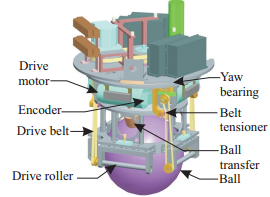
\includegraphics[width=5cm]{./Bilder/Markus/first_ballbot.png} }}%
	\qquad \qquad
	\subfloat[Ballbot der CMU entwickelt 2006.]{{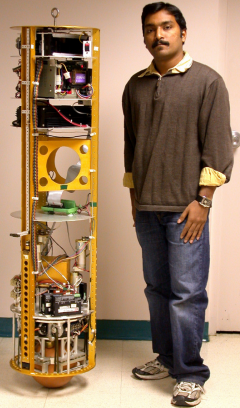
\includegraphics[width=3cm]{./Bilder/Markus/first_ballbot_human.png} }}%
	\caption{Aufbau Skizze und menschengro�er erster Ballbot \cite{umashankar_ballbot}. }%
	\label{fig:ballbot_cmu}%
\end{figure}

Dieser erste Ballbot ben�tigt mit vier bzw. f�nf Motoren sehr viele Ressourcen. 2009  stellte M. Kumaga \cite{kumaga} einen Ballbot, siehe Abbildung \ref{fig:omni_ballbots} (a), der durch drei omnidirektionale R�der angetrieben wird, vor. Dieser Ballbot kann sich ebenfalls um seine eigene Achse drehen und sogar eine Last von mindestens $10$\,{kg} tragen.

2010 stellte die Eidgen�ssische Technische Hochschule Z�rich (ETHZ) den Rezero vor \cite{ETHZ}, siehe Abbildung \ref{fig:omni_ballbots} (b). Dies ist ebenfalls ein Ballbot der mittels drei omnidirektionalen R�dern angetrieben wird. Er hat eine hohe dynamische Performanz und kann somit einen Neigungswinkel von bis zu $20$\,$^\circ$ ausregeln, sowie eine maximale lineare Geschwindigkeit von $2$\,m/s erreichen.

\begin{figure}[!htbp]%
	\centering
	\subfloat[Ballbot der Tohoku Gakuin Universit�t (2009) \cite{kumaga}. ]{{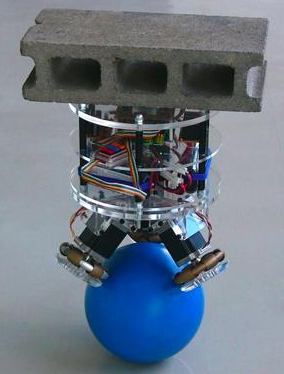
\includegraphics[width=3.5cm]{./Bilder/Markus/tgu_ballbot.png} }}%
	\qquad \qquad
	\subfloat[Ballbot Rezero der ETHZ (2010)  \cite{ETHZ}.]{{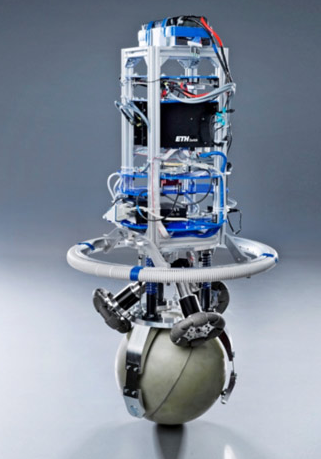
\includegraphics[width=3.5cm]{./Bilder/Markus/ethz.png} }}%
	\caption{Omnidirektionale Ballbot's der TGU und der ETHZ.}%
	\label{fig:omni_ballbots}%
\end{figure}

Inspiriert durch diese erfolgreichen Beispiele balancierender Roboter, soll in diesem Projektseminar ein Ballbot aufgebaut werden. Prim�res Ziel war das  Balancieren des Roboters auf einem Ball zu erreichen.

Die Umsetzung umfasste dabei den mechanischen Aufbau (Kap. \ref{ch:konstruktion}), die mathematische Modellierung (Kap. \ref{ch:Modellierung}), die Simulation (Kap. \ref{ch:Simulation}) und die Implementierung (Kap. \ref{ch:Implementierung}).